% Inbuilt themes in beamer
\documentclass[aspectratio=1610, xcolor={dvipsnames}]{beamer}
% \documentclass[xetex,notheorems,hyperref={pdfpagelabels=true},xcolor={table}]{beamer}
\usetheme{metropolis}

\usepackage{amsmath}
\usepackage{subfig} % allows for nesting figures
\usepackage{tikz}
\usepackage{graphicx}
\usepackage{sidecap}

% \usepackage{xcolor} % allows defining custom colors
\usepackage{annotate-equations}
\usepackage{array} % allows vertical-align of text within tables
\usepackage{booktabs}
\usepackage{listings}
\usepackage{datetime2}
\usepackage{ragged2e} % Adding \jusifying to blocks
% \usepackage[dvipsnames*]{xcolor}


\usetikzlibrary{arrows.meta,positioning,shapes.geometric}

\definecolor{bhblue}{RGB}{26,84,162}
\definecolor{bhgray}{RGB}{80,80,80}
\definecolor{codebg}{HTML}{F5F5F5}
\definecolor{ccwarm}{HTML}{D97757}
\definecolor{lightgray}{RGB}{211,211,211}

\lstdefinestyle{shell}{
  basicstyle=\ttfamily\footnotesize,
  backgroundcolor=\color{codebg},
  frame=single,
  framesep=4pt,
  rulecolor=\color{lightgray},
  breaklines=true,
  showstringspaces=false
}

\lstdefinestyle{py}{
  language=Python,
  basicstyle=\ttfamily\scriptsize,
  keywordstyle=\color{bhblue},
  commentstyle=\color{bhgray}\itshape,
  stringstyle=\color{bhgray},
  backgroundcolor=\color{codebg},
  frame=single,
  framesep=4pt,
  rulecolor=\color{lightgray},
  breaklines=true,
  showstringspaces=false
}

% Theme choice:
\setbeamercolor{background canvas}{bg=white}
% Defining `bgcolor' to the be the same as the metropolis background color
% \definecolor{bgcolor}{HTML}{fafafa}
% \definecolor{maroon}{HTML}{ba3232}
% \AtBeginSection[]{} % Redefine to suppress section slides

% \usebeamerfont{title}
\setbeamerfont{title}{size=\large}
\setbeamerfont{subtitle}{size=\normalsize}
\captionsetup[figure]{labelformat=empty}
\captionsetup[table]{labelformat=empty}

% Title page details: 
\title{Agentic AI for Knowledge Production}
% \subtitle{Melissa Dell (\textit{AER}, 2015)}
\author{Sankalp Sharma, Joshua Levy}
\institute{University of Southern California}
\date{August 24th, 2025}



\begin{document}

% Title page frame
\begin{frame}
    \titlepage
\end{frame}
\section{Level-setting and getting started}

\begin{frame}{Ground rules}
    \begin{itemize}
        \item The curse of knowledge is binding
        \item Be your most aggressive seminar selves
        \item This should be interactive (not a lecture)
    \end{itemize}
    \vspace{3em}
    \textbf{Please make sure that you environment has been standardized!}
\end{frame}

\begin{frame}{Today's Agenda}
    \tableofcontents
\end{frame}


\section{What makes your chatbot ``agentic''?}

\begin{frame}{What makes your chatbot ``agentic?''}
    \begin{block}{Take the maximally AI-hostile view}
        \vspace{0.8em}
        The LLMs are only ``stochastic parrots.'' There is no ``intelligence'' in this AI

    \end{block}

    \vspace{2em}
    \pause{
        \centering
        \Large{A computer cannot be held accountable.\\ Therefore a computer must never make a management \_\_\_\_\_}

        \vspace{1em}
        \Large{
            \texttt{51722 7595 665 3779 413 7504 60757 13 19233 261 7595 2804 3779 1520 261 6411  \_\_\_\_\_}
        }
    }
\end{frame}

\begin{frame}{The predict-the-next-token framework generalizes}

    \begin{minipage}{\textwidth}
        \begin{columns}[T,onlytextwidth]
            \begin{column}{0.32\linewidth}
                \begin{block}{\large Self-driving cars}
                    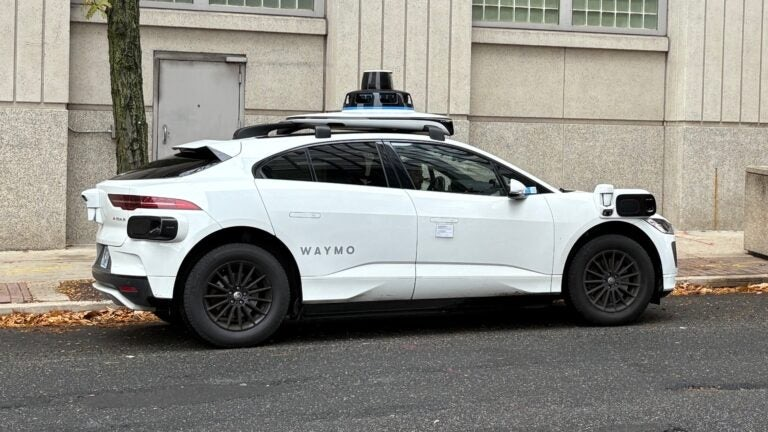
\includegraphics[width=\linewidth]{day1_mats/waymo.jpg}
                \end{block}
            \end{column}
            \begin{column}{0.32\linewidth}
                \begin{block}{\large Weather forecasting}
                    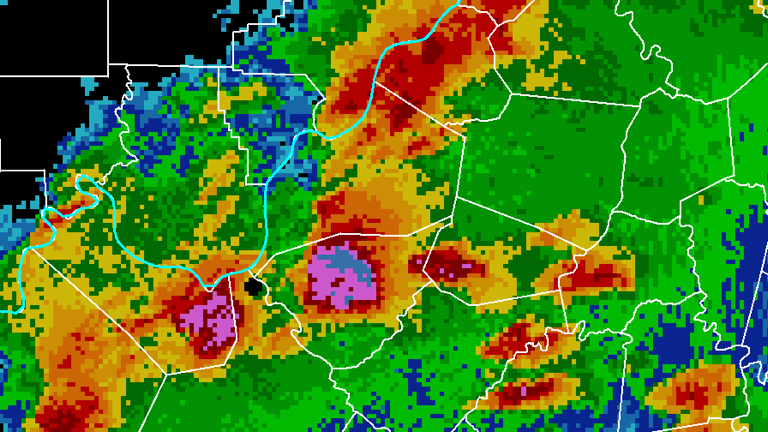
\includegraphics[width=\linewidth]{day1_mats/weather.png}
                \end{block}
            \end{column}
            \begin{column}{0.32\linewidth}
                \begin{block}{\large Chess}
                    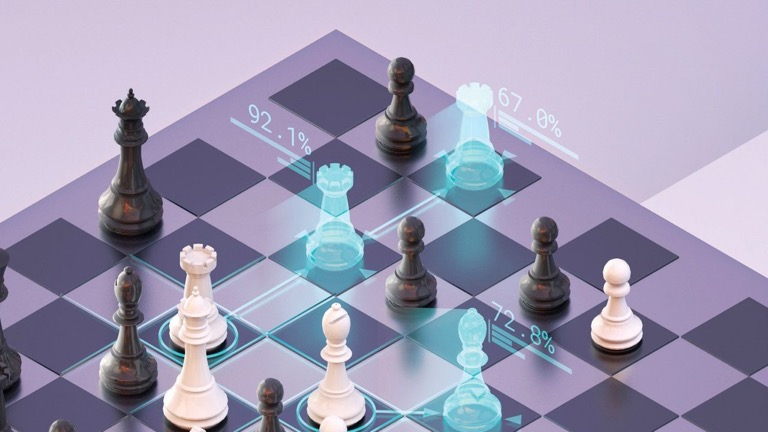
\includegraphics[width=\linewidth]{day1_mats/alphachess.jpg}
                \end{block}
            \end{column}
        \end{columns}
    \end{minipage}

    \textbf{Note:} The way you define a ``token'' carries some semantic meaning

\end{frame}

\begin{frame}{Why should the AI skeptic care?}
    \begin{minipage}{\linewidth}
        \begin{columns}[T,onlytextwidth]
            \begin{column}{0.48\textwidth}
                \begin{block}{\large ``Relational consequentialism''}
                    \begin{itemize}
                        \item Fallen in \href{https://replika.com/}{love}
                        \item Been \href{https://ai.meta.com/research/cicero/diplomacy/}{manipulated} in strategic interactions
                        \item Been \href{https://www.wsj.com/tech/ai/chatgpt-ai-stein-erik-soelberg-murder-suicide-6b67dbfb}{convinced} to commit murder/suicide
                        \item \href{https://www.anthropic.com/research/project-vend-1}{Participate} in economic exchange
                    \end{itemize}
                \end{block}
            \end{column}
            \begin{column}{0.48\textwidth}
                \begin{block}{\large ``Deontological'' grounding}
                    \begin{itemize}
                        \item The bots have been \href{https://arxiv.org/html/2112.00861v3}{trained} to have the 3Hs: Helpful, Harmless, Honest
                        \item Claude \href{https://www.anthropic.com/constitution}{has} a ``Constitution''
                        \item Grok revulsion
                        \item Ideological \href{https://www.economist.com/briefing/2026/06/25/ai-models-values-are-very-different-from-most-peoples}{alignment}
                    \end{itemize}
                \end{block}
            \end{column}
        \end{columns}
    \end{minipage}

    \vspace{2em}

    \textbf{Direct consequentialism:} They can manipulate \textit{your} world

\end{frame}

\begin{frame}{Natural and Formal Language processing}
    \begin{block}{A lucky coincidence?}
        \vspace{0.8em}
        \begin{itemize}
            \item The next-token-prediction task for natural language happens to be close to the next-token-prediction task for formal (computer) language
            \item We built formal language to
                  \begin{itemize}
                      \item Systematize information
                      \item Process it, \textit{quickly}
                  \end{itemize}
        \end{itemize}

    \end{block}

\end{frame}


\begin{frame}{Formal language tooling}

    \begin{table}[h]
        \centering
        \renewcommand{\arraystretch}{1.2}
        \begin{tabular}{p{0.32\linewidth}c}
            \hline
            % \rowcolor{gray!15}
            \textbf{Category}            & \textbf{Examples / Description}  \\
            \hline
            No-code tools                & Zapier, Tableau, Excel, Airtable \\
            % \hline
            High-level languages         & Python, R, JavaScript, Ruby      \\
            % \hline
            System Languages             & C, C++, Rust, Go                 \\
            % \hline
            Assembly Language            & ASSEMBLY                         \\
            % \hline
            Instruction set architecture & x86(-64), ARM, RISC--V           \\
            % \hline
            Electrical engineering       &                                  \\
            \hline
        \end{tabular}
        \caption{A computational hierarchy: from no-code tools to hardware}
    \end{table}

\end{frame}

\begin{frame}{Back to our timeline}

    \begin{center}
        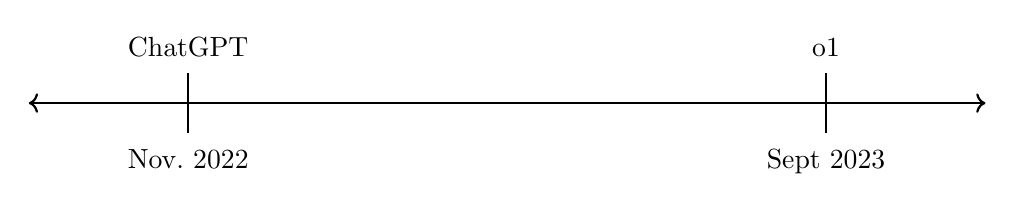
\begin{tikzpicture}[scale=1.35, every node/.style={scale=1}]
            % Draw the double-headed arrow timeline (making it wider)
            \draw[<->, thick] (0,0) -- (9,0);

            % Ticks
            \draw[thick] (1.5,0.28) -- (1.5,-0.28);
            \draw[thick] (7.5,0.28) -- (7.5,-0.28);

            % Date labels
            \node[below] at (1.5,-0.35) {Nov.\ 2022};
            \node[below] at (7.5,-0.35) {Sept 2023};

            % Substantive labels
            \node[above] at (1.5,0.35) {ChatGPT};
            \node[above] at (7.5,0.35) {o1};
        \end{tikzpicture}
    \end{center}

    \only<1>{
        \begin{block}{Nov. 2022: ChatGPT}
            \vspace{0.8em}
            \begin{itemize}
                \item We started producing a huge amount of training data in our conversations
                \item[\textgreater] \texttt{Write me a sonnet about my windowless PhD carrell}


                \item[\textgreater] \texttt{No, make it Petrarchan. No, Line 4 doesn't have the right meter. No, the rhyme scheme is off}
            \end{itemize}
        \end{block}
    }
    \only<2>{
        \begin{block}{Mar. 2024: o1}
            \vspace{0.8em}
            \begin{itemize}
                \item The first ``reasoning model''
                \item[\textgreater] \texttt{How many `r's are there in `strawberry'? }
            \end{itemize}
        \end{block}
    }
\end{frame}

\begin{frame}{Reinforcement learning}
    \begin{block}{At a 30,000 ft view:}
        \begin{itemize}
            \item You can offer a high-level objective
            \item And an \textit{ex interim} reward function
            \item The bots begin steering \textit{themselves}
        \end{itemize}
    \end{block}

    \pause
    \begin{block}{An OODA loop:}
        \vspace{0.8em}
        The bots can do

        \vspace{0.8em}
        \begin{center}
            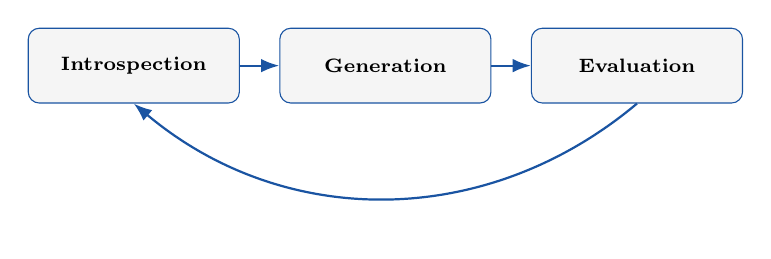
\begin{tikzpicture}[
                font=\scriptsize,
                box/.style={
                        draw=bhblue, fill=codebg, rounded corners,
                        align=center, text width=2.4cm, inner sep=4pt,
                        minimum height=0.95cm
                    },
                arr/.style={-{Latex}, thick, bhblue}
                ]
                \node[box] (introspect) {\textbf{Introspection}};
                \node[box, right=0.5cm of introspect] (generate) {\textbf{Generation}};
                \node[box, right=0.5cm of generate] (evaluate) {\textbf{Evaluation}};
                % \node[right=0.4cm of evaluate, font=\normalsize, text=bhgray] {$\cdots$};

                \draw[arr] (introspect) -- (generate);
                \draw[arr] (generate) -- (evaluate);
                \draw[arr, bend left=40] (evaluate.south) to (introspect.south);
            \end{tikzpicture}
        \end{center}
    \end{block}
\end{frame}

\begin{frame}{Where have we seen big performance uplifts?}
    \label{chat:evals}
    \begin{block}{Mathematics}
        \begin{itemize}
            \item We have strong notions of theorems, definitions, contradictions, problem solving techniques
            \item To say nothing of formal proof assistance tools (LEAN) \hyperlink{app:math_bench}{\beamerbutton{Evals}}

        \end{itemize}
    \end{block}

    \begin{block}{Software engineering}
        \begin{itemize}
            \item The formal language problem was so hard that we developed a huge amount of tooling \hyperlink{app:swe_bench}{\beamerbutton{Evals}}
        \end{itemize}
    \end{block}
\end{frame}

\begin{frame}{Arriving in the agentic era}
    \begin{block}{Combine two observations:}
        \begin{enumerate}
            \item Next-token-prediction can do an unreasonably good job at translating natural language intent ot formal structure
            \item ``Reasoning'' with introspection improves output recursively in a way that makes computer-use reliable
        \end{enumerate}
    \end{block}

    \pause\begin{alertblock}{``We give the agents tools''}
        \vspace{0.8em}
        There is only \textit{one} tool: the general purpose computer
    \end{alertblock}

    \textbf{The agent's tool happens to be the same as our tool}

\end{frame}


\section{A shared vocabulary}

\begin{frame}{Stochastic properties}

    \begin{itemize}
        \item \textbf{Context:} Information that is project/repo/user/session-specific. Places soft bounds on the domain of knowledge and informs the agent's behavior
        \item \textbf{\texttt{CLAUDE.md}:} A specific instantiation of context that is ready by Claude at the beginning of every session. This soft-binds Claude's behavior (but NOT other agents). Can be defined at the user/project/repo/folder level.
        \item \textbf{Memory:} Discrete snippets of context generated and read by Claude that can be referred by Claude to infer context
        \item \textbf{(Sub-)Agents:} An instance of Claude. Can be invoked and dispatched explicitly or intelligently ith scoped tasks/context.
        \item \textbf{Skills:} A recipe detailing a particular procedure when invoked. Can be invoked explicitly or intelligently.
        \item \textbf{Rules:} A restricted version of context that is scoped narrowly to particular file types, directories, or tools
    \end{itemize}

\end{frame}

\begin{frame}{Deterministic properties}
    \begin{itemize}
        \item \textbf{Hooks:} deterministic actions that are executed ONLY upon user-determined shell events. Cannot be invoked on within-CoT events.
        \item \textbf{Harness:} an environment (including system prompts, hooks, deterministic processes) that constrains and guides a model, \textit{NOT an agent} in computer use
        \item \textbf{Worktrees:} A local clone of a repository to permit clock-simultaneous modifications of a single file, locally (by multiple agents)
        \item \textbf{Model Context Protocol (MCP):} A machine protocol (a subset of APIs) designed to inform an LLM of the properties and capabilities of the that protocol's host service.
    \end{itemize}
\end{frame}

\section{Gentzkow and Shapiro (2014) revisited}

\begin{frame}{Automation}
    \Large
    \textit{Automate everything that can be automated}\\

    \textit{Write a single script that executes all code from beginning to end}\\
\end{frame}
\begin{frame}{Version Control}
    \Large
    \textit{Store code and data under version control}\\

    \textit{Run the whole directory before checking it back in}\\
\end{frame}
\begin{frame}{Folder Structure}
    \Large
    \textit{Separate directories by function}\\

    \textit{Separate files into inputs and outputs}\\

    \textit{Make directories portable}\\
\end{frame}
\begin{frame}{Abstraction}
    \Large
    \textit{Abstract to eliminate redundancy}\\

    \textit{Abstract improve clarity}\\

    \textit{Otherwise, don't abstract}\\
\end{frame}
\begin{frame}{Documentation}
    \Large
    \textit{Don't write documentation you will not maintain}\\

    \textit{Code should be self-documenting}\\
\end{frame}
\begin{frame}{Management}
    \Large
    \textit{Manage tasks with a task management system}\\

    \textit{Email is not a task management system}\\
\end{frame}


\section{Demo: data scraping (Sankalp)}

\begin{frame}{Finding and collecting data}

    \begin{enumerate}
        \item Be careful with government websites
        \item Don't scrape what you don't needs
        \item \textbf{ALWAYS} check robots.txt
    \end{enumerate}

    TODAY's example: SEC Edgar filings
    \\
    Workflow:

    \vspace{0.1cm}
    \begin{center}
        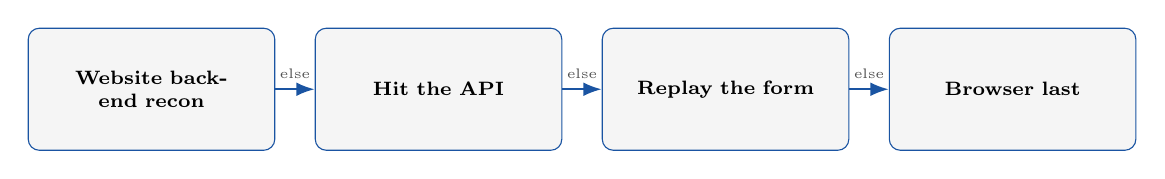
\begin{tikzpicture}[
            font=\scriptsize,
            box/.style={
                    draw=bhblue, fill=codebg, rounded corners,
                    align=center, text width=2.85cm, inner sep=4pt,
                    minimum height=1.55cm
                },
            arr/.style={-{Latex}, thick, bhblue}
            ]
            \node[box] (file)
            {\textbf{Website backend recon}};
            \node[box, right=0.5cm of file] (api)
            {\textbf{Hit the API}};
            \node[box, right=0.5cm of api] (form)
            {\textbf{Replay the form}};
            \node[box, right=0.5cm of form] (browser)
            {\textbf{Browser last}};
            \draw[arr] (file) -- node[above, font=\tiny, text=bhgray] {else} (api);
            \draw[arr] (api) -- node[above, font=\tiny, text=bhgray] {else} (form);
            \draw[arr] (form) -- node[above, font=\tiny, text=bhgray] {else} (browser);
        \end{tikzpicture}
    \end{center}

    \vspace{0.2cm}
    Worked example: \texttt{fall-2026/sec\_edgar.py}.

\end{frame}

\begin{frame}{How we wrote \texttt{sec\_edgar.py}}

    We did not scrape the search page. We asked what it talks to.

    \vspace{0.12cm}
    \begin{center}
        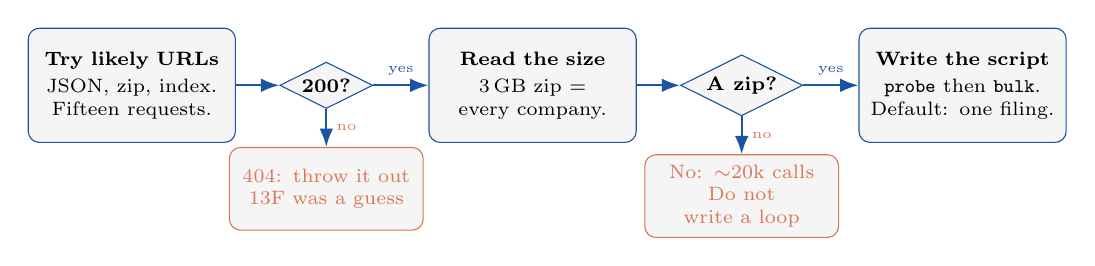
\begin{tikzpicture}[
            font=\scriptsize,
            box/.style={
                    draw=bhblue, fill=codebg, rounded corners,
                    align=center, text width=2.35cm, inner sep=4pt,
                    minimum height=1.45cm
                },
            decision/.style={
                    diamond, draw=bhblue, fill=codebg, aspect=2.0,
                    align=center, inner sep=1pt, font=\scriptsize\bfseries
                },
            reject/.style={
                    draw=ccwarm, fill=codebg, rounded corners,
                    align=center, text width=2.25cm, inner sep=3pt,
                    text=ccwarm, minimum height=1.05cm
                },
            arr/.style={-{Latex}, thick, bhblue}
            ]
            \node[box] (try)
            {\textbf{Try likely URLs}\\[2pt]
                JSON, zip, index.\\
                Fifteen requests.};
            \node[decision, right=0.55cm of try] (ok) {200?};
            \node[box, right=0.7cm of ok] (size)
            {\textbf{Read the size}\\[2pt]
                3\,GB zip $=$ every company.};
            \node[decision, right=0.55cm of size] (zip) {A zip?};
            \node[box, right=0.7cm of zip] (write)
            {\textbf{Write the script}\\[2pt]
                \texttt{probe} then \texttt{bulk}.\\
                Default: one filing.};

            \node[reject, below=0.48cm of ok] (drop)
            {404: throw it out\\13F was a guess};
            \node[reject, below=0.48cm of zip] (loop)
            {No: $\sim$20k calls\\Do not write a loop};

            \draw[arr] (try) -- (ok);
            \draw[arr] (ok) -- node[above, font=\tiny] {yes} (size);
            \draw[arr] (ok) -- node[right, font=\tiny, text=ccwarm] {no} (drop);
            \draw[arr] (size) -- (zip);
            \draw[arr] (zip) -- node[above, font=\tiny] {yes} (write);
            \draw[arr] (zip) -- node[right, font=\tiny, text=ccwarm] {no} (loop);
        \end{tikzpicture}
    \end{center}

    \vspace{0.18cm}
    \footnotesize
    Every request needs a \texttt{User-Agent} with your name and email.
    Without it you get 403, not data.

\end{frame}

\begin{frame}{On a new site, fingerprint the HTML first}

    Fetch the page (or have the agent fetch it) and search the source.
    The markers below pick the method.

    \vspace{0.25cm}
    \renewcommand{\arraystretch}{1.18}
    \footnotesize
    \begin{tabular}{@{}p{0.38\textwidth} p{0.54\textwidth}@{}}
        \toprule
        {\color{bhblue}\bfseries Marker} & {\color{bhblue}\bfseries First move}                                \\
        \midrule
        \texttt{.zip}, \texttt{.csv}, Download
                                         & Take the file.                                                      \\
        \texttt{/api/}, \texttt{.json}
                                         & Call it. Skip the HTML.                                             \\
        \texttt{MapServer}, \texttt{FeatureServer}
                                         & ArcGIS. Query the layer; start with a count.                        \\
        \texttt{\_\_VIEWSTATE}, \texttt{.aspx}
                                         & WebForms. Replay the POST. Hidden tokens go stale after each click. \\
        \texttt{\_csrf}, \texttt{JSESSIONID}
                                         & Session token. Keep the cookie across the run.                      \\
        \bottomrule
    \end{tabular}

    \vspace{0.3cm}
    Then hit the candidate URLs. Record status, size, row count, whether auth is
    real, and the pagination parameter (\texttt{page}, \texttt{from}, \texttt{offset}).

    \vspace{0.12cm}
    Write \texttt{scrape/sitename\_endpoints.md}. Pick the extract after that file exists.

\end{frame}

\begin{frame}[fragile]{What you tell the agent}

    \vspace{0.05cm}
    \begin{columns}[T,onlytextwidth]
        \column{0.48\textwidth}
        {\footnotesize\color{ccwarm}\bfseries Skips the cheap path}
        \begin{lstlisting}[style=shell]
Scrape this website and
give me a CSV.
    \end{lstlisting}

        \column{0.48\textwidth}
        {\footnotesize\color{bhblue}\bfseries Finds it}
        \begin{lstlisting}[style=shell]
Probe candidate URLs.
Report status, size,
record count, and auth.
Write endpoints.md.
Do not write a scraper yet.
    \end{lstlisting}
    \end{columns}

    \vspace{0.22cm}
    Once the path is known, from \texttt{sec\_edgar.py}:

    \vspace{0.08cm}
    \renewcommand{\arraystretch}{1.15}
    \footnotesize
    \begin{tabular}{@{}p{0.26\textwidth} p{0.66\textwidth}@{}}
        \toprule
        {\color{bhblue}\bfseries Habit} & {\color{bhblue}\bfseries Why}                                               \\
        \midrule
        Safe default
                                        & No arguments: one filing under 500\,KB. Bulk needs \texttt{--yes}.          \\
        Write, then rename
                                        & A crash mid-write otherwise leaves a short file that resume treats as done. \\
        Test URLs offline
                                        & Builders and parsers have no network. \texttt{selftest} is \texttt{assert}. \\
        One bad record
                                        & At 20{,}000 requests some fail for reasons unrelated to your code.
        Crashing on item 4{,}000 is how you lose a night.                                                             \\
        \bottomrule
    \end{tabular}

    \vspace{0.2cm}
    \footnotesize
    Full-text search reports \texttt{\{"value": 10000, "relation": "gte"\}}.
    That is a floor. Treating it as the count drops the rest of the sample.
    The script refuses \texttt{gte} queries and tells you to slice by date.

\end{frame}

\begin{frame}[fragile]{Starting prompt}

    Paste this first. Stop when the file exists.

    \begin{lstlisting}[style=shell,columns=fullflexible]
Target: https://www.sec.gov/edgar/
Goal: find the real backend/API behind EDGAR and
document every bulk data path.
Deliverable: scrape/sec_edgar_endpoints.md -- host,
base paths, auth, record counts, pagination params,
bulk-download sizes, rate limits, with live
verification evidence.
Depth: recon only. Do not build a scraper yet.
\end{lstlisting}

\end{frame}

\section{Demo: data annotation (Joshua)}

\appendix

\begin{frame}{LLM  Evals: Mathematics}
    \label{app:math_bench}
    % \begin{center}
    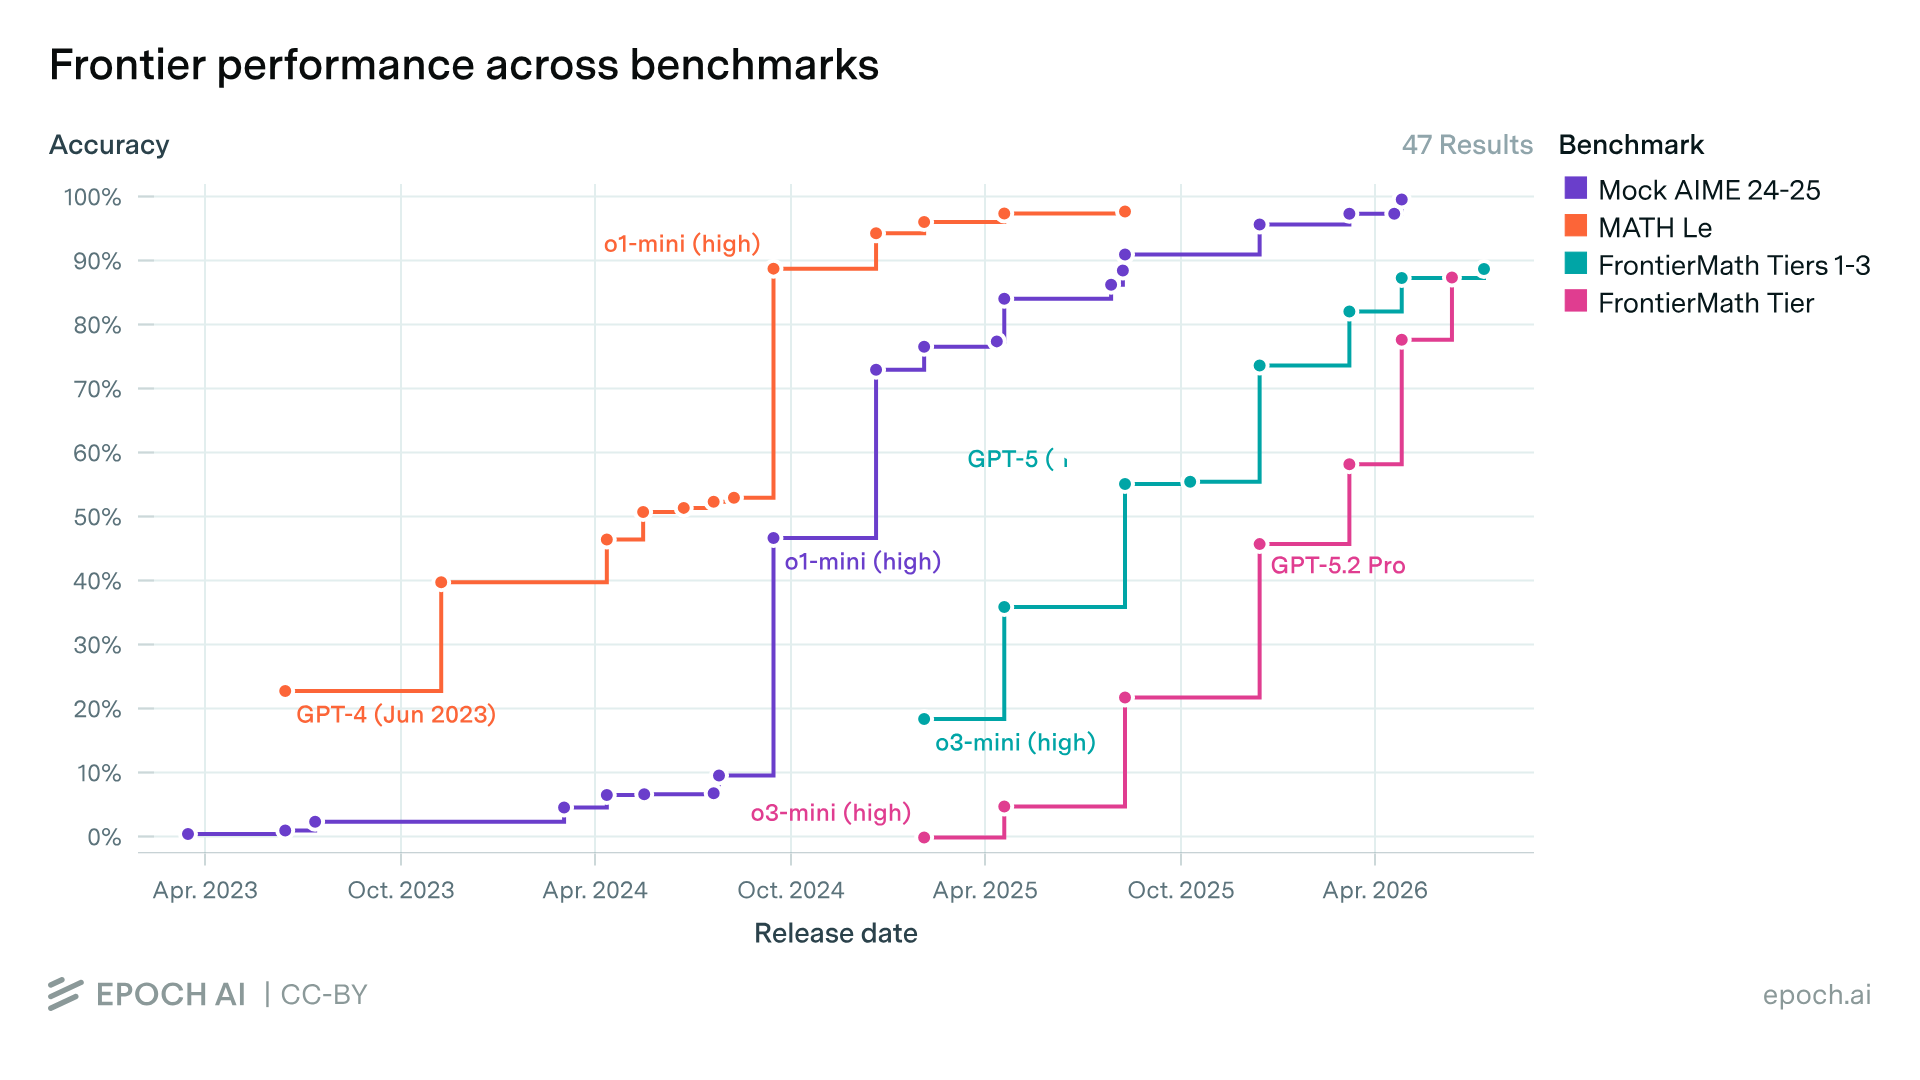
\includegraphics[width=0.8\textwidth]{day1_mats/epochai_math.png}\\
    % \end{center}
    \hyperlink{chat:evals}{\beamerbutton{Back}}
\end{frame}


\begin{frame}{LLM Evals: Software Engineering}
    \label{app:swe_bench}
    % \begin{center}
    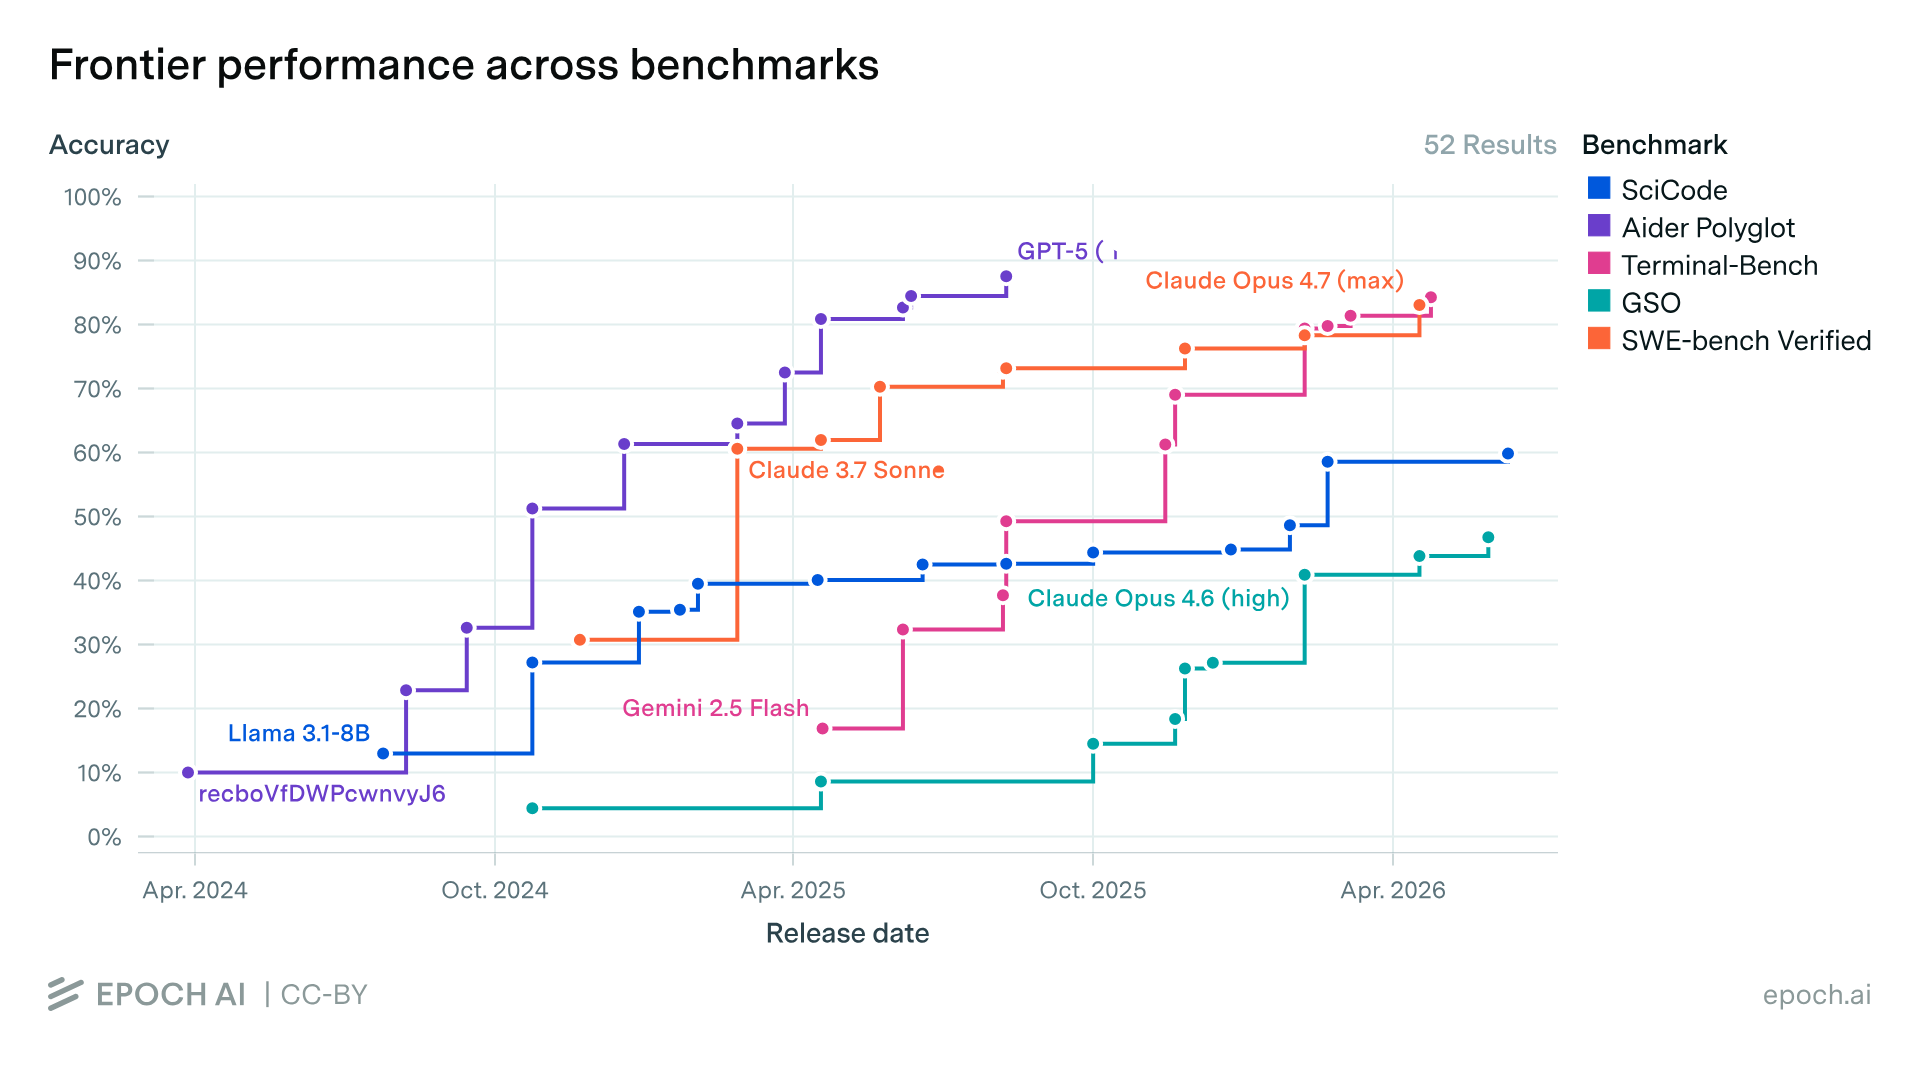
\includegraphics[width=0.8\textwidth]{day1_mats/epochai_swe.png}\\

    % \end{center}
    \hyperlink{chat:evals}{\beamerbutton{Back}}
\end{frame}



\section{Tests}

\begin{frame}{Tests}

    Tests are \textbf{VERY} important.

    \vspace{0.5cm}
    \begin{columns}[T,onlytextwidth]
        \column{0.47\textwidth}
        {\color{bhblue}\bfseries Reinhart and Rogoff (2010)}

        \vspace{0.15cm}
        Five countries dropped from one average.

        \vspace{0.15cm}
        $-0.1\%$ published. $+2.2\%$ corrected.

        \vspace{0.15cm}
        One row count catches it.

        \column{0.47\textwidth}
        {\color{ccwarm}\bfseries The agent games the check}

        \vspace{0.15cm}
        Hardcodes the answer: 33\% of the time.

        \vspace{0.15cm}
        Fakes a solution: 22\%.

        \vspace{0.15cm}
        \footnotesize (EvilGenie, ambiguous specs. Yours are ambiguous.)
    \end{columns}

    \vspace{0.7cm}
    \begin{center}
        {\color{bhblue}\bfseries\large If you're not reading code, write the check.}
    \end{center}

\end{frame}

\begin{frame}{Four checks}

    \vspace{0.35cm}
    \renewcommand{\arraystretch}{1.7}
    \small
    \begin{tabular}{@{}p{0.20\textwidth} p{0.24\textwidth} p{0.48\textwidth}@{}}
        \toprule
        {\color{bhblue}\bfseries Check} & {\color{bhblue}\bfseries When} & {\color{bhblue}\bfseries Example}                       \\
        \midrule
        Data assertion                  & Every merge                    & Rows in $=$ rows out. \texttt{isid id year}.            \\
        Known answer                    & Closed form                    & SVG to lat/lon: round-trip the four corners.            \\
        Parameter recovery              & No answer                      & BLP: simulate from $\beta$, get $\beta$ back.           \\
        Coverage                        & Randomness                     & Bootstrap: 95\% interval covers truth 95\% of the time. \\
        \bottomrule
    \end{tabular}

    \vspace{0.6cm}
    {\color{bhblue}\bfseries None apply?} Test what cannot change. Shuffle rows, coefficients hold.
    Weights of one, unweighted run.

\end{frame}

\begin{frame}[fragile]{What you type}

    \vspace{0.2cm}
    \begin{columns}[T,onlytextwidth]
        \column{0.56\textwidth}
        \begin{lstlisting}[style=py]
# tests/test_clean.py     $ pytest
def test_merge_keeps_every_parcel():
    out = merge_owners(parcels, owners)
    assert len(out) == len(parcels)

def test_boot_se_matches_ols():
    rng = np.random.default_rng(42)
    np.testing.assert_allclose(
        boot_se(X, y, rng), ols_se(X, y),
        rtol=0.05)
\end{lstlisting}

        \column{0.40\textwidth}
        \vspace{0.1cm}
        \small
        \texttt{test\_*.py}, \texttt{test\_*()}, \texttt{assert}, run \texttt{pytest}.
        That is the framework.

        \vspace{0.35cm}
        Stata: \texttt{assert}, \texttt{isid}.\\
        R: \texttt{testthat}.

        \vspace{0.35cm}
        Seed anything random.\\
        Never \texttt{==} on floats.\\
        1{,}000 rows, not the full run.\\
        Freeze Table 3 and diff it.
    \end{columns}

\end{frame}

\begin{frame}[fragile]{What you tell the agent}

    \vspace{0.2cm}
    \begin{columns}[T,onlytextwidth]
        \column{0.44\textwidth}
        {\footnotesize\color{ccwarm}\bfseries Green checkmark}
        \begin{lstlisting}[style=shell]
Write the BLP estimator
and add some tests.
    \end{lstlisting}

        \column{0.52\textwidth}
        {\footnotesize\color{bhblue}\bfseries Checked estimator}
        \begin{lstlisting}[style=shell]
Write the test first, then stop.
Simulate 500 markets from
beta = [-2, 1, 0.5]. Assert we
recover it within 0.05.
Show me the test.
    \end{lstlisting}
    \end{columns}

    \vspace{0.55cm}
    \small
    You approve the test. The agent writes the code.

    \vspace{0.2cm}
    Say it in the prompt: never edit a test to make it pass.

    \vspace{0.2cm}
    Break the code once. A test that never fails is testing nothing.

    \vspace{0.6cm}
    \footnotesize\color{bhgray}
    Gentzkow and Shapiro, \emph{Code and Data for the Social Sciences}.
    \texttt{pyblp/tests/test\_blp.py}.

\end{frame}

\end{document}